% The inverse operator bound converts residual differences to trajectory differences.
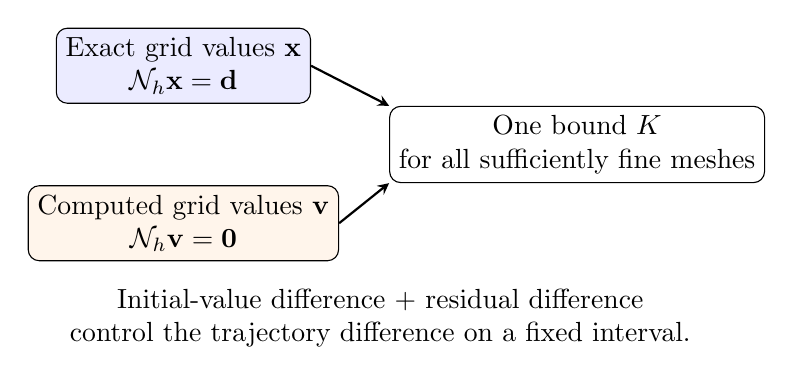
\begin{tikzpicture}[>=stealth,font=\normalsize,box/.style={draw,rounded corners,align=center,minimum height=.8cm}]
\node[box,fill=blue!8](a)at(0,1){Exact grid values $\mathbf x$\\$\mathcal N_h\mathbf x=\mathbf d$};
\node[box,fill=orange!8](b)at(0,-1){Computed grid values $\mathbf v$\\$\mathcal N_h\mathbf v=\mathbf0$};
\node[box](c)at(5,0){One bound $K$\\for all sufficiently fine meshes};
\draw[->,thick](a.east)--(c.north west);\draw[->,thick](b.east)--(c.south west);
\node[align=center]at(2.5,-2.2){Initial-value difference + residual difference\\control the trajectory difference on a fixed interval.};
\end{tikzpicture}
